\chapter{Introduction}  \label{Sec:Intro}


In this chapter, we introduce the phase retrieval problem and summarize the goals of this dissertation.
Section \ref{Subsec:phase_retrieval-math_model} defines the phase retrieval problem.
Section \ref{Subsec:phase_retrieval-applications} describes a common phase retrieval application and presents the experimental model which we use throughout this dissertation for numerical testing.
Section \ref{Subsec:Intro-contributions} describes the contributions and layout of this dissertation.
Finally, Section \ref{Subsec:Intro-notation} defines the notation used in this dissertation.


\section{Phase Retrieval}	\label{Subsec:phase_retrieval-math_model}



Phase retrieval is the problem of recovering a signal from magnitude-only observations with little or no knowledge of the signal phase.  
Let $\mathbf{x}$ be a desired signal (or \textit{true signal}) in $\bbR^n$ or $\bbC^n$ which as been observed with sensing (or sampling) vectors $a_i \in \bbC^n$, resulting in squared measurements $|\langle a_i, \mathbf{x} \rangle |^2 = \mathbf{b}_i \in \bbR$ for $i = 1, \ldots, m$.
Also assume the \textit{true observation} vector $\mathbf{b} = [\mathbf{b}_1, \ldots, \mathbf{b}_m]^T \in \bbR^m$ has been contaminated by possibly nontrivial noise $\eta = [\eta_1, \ldots, \eta_m]^T \in \bbR^m$, giving the observation vector $b = \mathbf{b} + \eta \in \bbR^m$.  Then we define the \textit{phase retrieval problem} as
\begin{equation} \label{Eqn:phase_retrieval}
\begin{array}{lll}
\textnormal{find}		&	x		\\
\st				&	|\langle a_i, x \rangle|^2 = b_i = \mathbf{b}_i + \eta_i	&	1 \leq i \leq m,
\end{array}
\end{equation}
where $x$ is an approximation of the desired signal $\textbf{x}$.  
Note that if $b$ is not identically zero then the solution $\textbf{x}$ will not be unique since we may change the sign or phase of $\textbf{x}$ to generate additional solutions.
If $\eta_i = 0$ for all $i$, then (\ref{Eqn:phase_retrieval}) is the noiseless phase retrieval problem (from \cite{Fienup82} and  \cite{DBLP:journals/tit/CandesLS15} among many others).  In this dissertation however, we are primarily concerned with nontrivial noise and will refer to (\ref{Eqn:phase_retrieval}) with $||\eta||_2 > 0$ as \textit{noisy phase retrieval}.  Additionally, we are concerned with noise $\eta$ which has a Gaussian distribution, as discussed in \cite{DBLP:journals/siamis/CandesESV13} and \cite{DBLP:journals/siamsc/FriedlanderM16}.


Each sensing vector $a_i \in \bbC^n$ is typically the conjugate of the $i$th row of the $n-$dimensional discrete Fourier transformation (DFT) matrix $F$ \cite[Chapter 11]{bracewell1986fourier}.  This gives the constraint $|Fx|^2 = b$ (where the square operator is applied element-wise).  Often the number of observations $m = nL$ is oversampled by a factor of $L$ to promote uniqueness of a signal solution and convergence of a given algorithm.  

The domain of the constraint in (\ref{Eqn:phase_retrieval}) is a high-dimensional torus, and thus phase retrieval is inherently nonconvex.  When deciding how to handle a particular phase retrieval problem, this  nonconvexity presents a unique challenge in terms of choosing an appropriate algorithm.  






\section{Applications and Experimental Models} 			\label{Subsec:phase_retrieval-applications}


Phase retrieval has a broad range of applications across the sciences, many of which fall into the general category of coherent diffraction imaging (CDI) \cite{miao1999extending}.  
This section provides a brief overview of CDI and closes with a description of the phase retrieval experimental models used in this dissertation (as well as \cite{DBLP:journals/siamis/CandesESV13}, \cite{DBLP:journals/tit/CandesLS15}, and \cite{DBLP:journals/siamsc/FriedlanderM16}).
More specific applications of phase retrieval can be found in astronomy \cite{fienup1987phase}, diffraction and array imaging \cite{bunk2007diffractive} \cite{chai2010array}, microscopy \cite{miao2008extending}, optics \cite{walther1963question}, and x-ray crystallography \cite{harrison1993phase}, \cite{millane1990phase} (for a recent benchmark set of crystallography problems, see \cite{elser2017benchmark}).  
For a comprehensive introduction to optical phase retrieval and an overview of recent theory and methods, see the survey \cite{DBLP:journals/spm/ShechtmanECCMS15}.


CDI is a method for reconstructing $2$- or $3$-dimensional nano-structures (e.g., nanotubes, nanocrystals, proteins).  In this process, highly coherent waves (e.g., x-rays, electrons, photons) are projected at a given object.  The resulting diffraction creates a pattern of intensities which are measured with a detector, resulting in magnitude-only measurements.  Figure \ref{Fig:CDI} below depicts the CDI observation process.

\begin{figure}
\centering
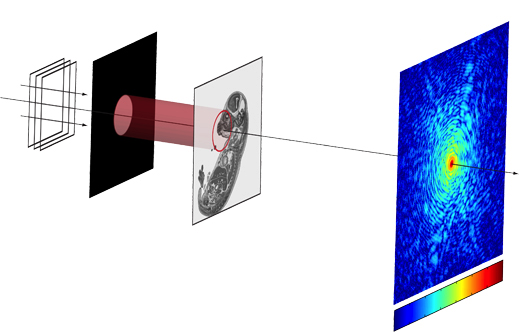
\includegraphics[width=0.75\textwidth]{phase_retrieval_depiction_mod.jpg}
   \caption{Depiction of coherent diffractive imaging.  Coherent waves (left) are projected at an image (center) which causes a diffraction pattern that is measured by a detector (right). Image from \cite{Guizar-Sicairos}.} 
   \label{Fig:CDI}
\end{figure}

Because CDI does not involve optical lenses, there is no optical aberration (blurring or distorting).  
Instead, the resolution depends on the limits of diffraction and dose.  
Many efficient methods exist for handling low-noise phase retrieval (see Chapter \ref{Sec:phase_retrieval} for an overview of some common methods).  
However, due to the nonconvexity of the constraints in (\ref{Eqn:phase_retrieval}), many low-noise methods lead to algorithms which are likely to diverge or converge to a suboptimal local minimum if there is modest noise or an insufficient number of observations.  
Thus accurate CDI typically requires minimal noise and multiple observations to recover a high-resolution solution.




When developing an experimental model, there are many methods for increasing the number of observations of a signal.  Some options include rotating the position of the object, using a spatial light modulator to defocus the observations, and inserting phase plates, or \textit{masks}, in line with the waves (see the survey \cite{duadi2011digital} for a discussion of these methods).  Our experimental models use the same masking method described in \cite[Section 2]{DBLP:journals/siamis/CandesESV13}, \cite[Sections 4.2, 4.3]{DBLP:journals/tit/CandesLS15}, and \cite[Section 5.1]{DBLP:journals/siamsc/FriedlanderM16} (see Section \ref{Subsubsec:phase_retrieval-unstructured} for an overview of these papers).  
This masking method involves placing a phase plate with a known structure oriented normal to the projected waves.  The phase plate can be placed on either side of the object; in our experiments, the plate lies between the object and the detector.  The mask is then shifted and multiple observations are collected.




Mathematically, the application of a phase plate to the phase problem (\ref{Eqn:phase_retrieval}) is equivalent to replacing the sensing operator $|Fx|^2$ with $|FC_jx|^2$, where the matrices $C_j \in \mathbb{C}^{n \times n}$ for $j = 1, \ldots, L$ are diagonal with standard Gaussian distribution entries $C_j(i,i) \sim \caN(0, 1)$, representing the diffraction patterns of the shifted phase plate.  This gives the observation constraint

\begin{equation}		\label{Eqn:FCx}
	\begin{vmatrix}
		FC_1x \\ \vdots \\ FC_Lx
	\end{vmatrix}^2
	= b.
\end{equation}

In certain cases only a limited number of observations can be collected.  For instance, in x-ray imaging, overexposure of the incident waves to the object (living tissue) can be dangerous.  Thus the number of observations $L$ may be relatively small compare to the signal size $n$, again making signal recovery difficult for nonconvex methods.





In this dissertation, our experimental phase retrieval models are generating using the method established in \cite{DBLP:journals/tit/CandesLS15} and extended in \cite{DBLP:journals/siamsc/FriedlanderM16}.  
We begin with a true signal $\mathbf{x}$ which is either a vectorized image or a randomly generated vector with coordinates having complex standard Gaussian distribution $\mathbf{x}_i \sim \caN(0, 1)$.
Next, we generate $j = 1, \ldots,  L$ diagonal mask matrices $C_j \in \mathbb{C}^{n \times n}$ with diagonal entries $C_j(i,i) \sim \caN(0, 1)$.
We then compute the product (\ref{Eqn:FCx}) to obtain the true observation vector $\mathbf{b}$.
For noiseless phase retrieval, we set the observation vector to $b = \mathbf{b}$.
If the phase retrieval problem requires a nonzero noise term $\eta$, we add $\eta$ to the true observation to obtain the observation vector $b = \mathbf{b} + \eta$.
Figure \ref{Fig:parrot_signal_iterates} below depicts the primary test image used in this dissertation.
Here, an original image of size $128 \times 128$ is used to generate a noisy phase retrieval problem, and we see a few particular iterates returned by the Gauge Dual Descent (GDD) algorithm, the primary algorithm considered in this dissertation (Algorithm \ref{Alg:PGD} in Section \ref{Subsec:PLGD_algo-algo}).  
For a complete explanation of our method for creating noisy phase retrieval problems, see Section \ref{Subsec:PLGD_term_crit-NOISY_MODELS_AND_RESIDUALS}.

\begin{figure}[H]
\centering
\hbox{\hspace{-2.55cm} 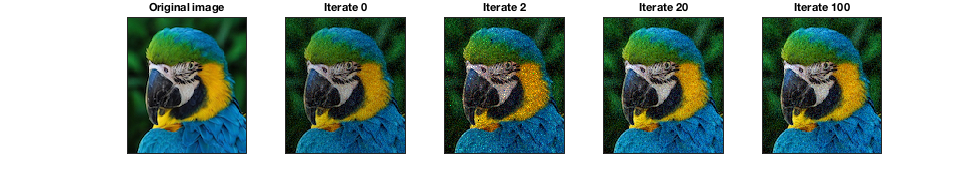
\includegraphics[scale=0.6]{parrot_signal_iterates} }
\caption{Results from the Gauge Dual Descent algorithm (Algorithm \ref{Alg:PGD} in Section \ref{Subsec:PLGD_algo-algo}) applied to a noisy phase retrieval problem (\ref{Eqn:phase_retrieval}) with oversampling rate $L = m/n=8$ and noise ratio $\epsilon_\text{rel} = ||\eta||_2 / ||b||_2 = 0.30$.}
\label{Fig:parrot_signal_iterates}
\end{figure}
% experiments.figure.noisyimage_signal_relerr_various_saga_iterates






\section{Contributions}		\label{Subsec:Intro-contributions}


We now summarize the contributions and layout of this dissertation.
As we will see in Chapter \ref{Sec:phase_retrieval}, a wide range of mathematical models and solution methods have been developed for phase retrieval.
Yet few models exist for noisy phase retrieval without imposing additional restrictions such as signal sparsity.  
One recent noisy phase retrieval model which requires no underlying assumptions is the gauge dual of the PhaseLift model (PLGD), which we define in Section \ref{Subsec:PLGD-models_intro}.



The PLGD model was first introduced and analyzed in \cite{DBLP:journals/siamsc/FriedlanderM16}, and is based on the PhaseLift model \cite{DBLP:journals/siamis/CandesESV13} in which a desired signal of $n$ elements (e.g., pixels) is lifted into the space of $n \times n$ positive semidefinite matrices, creating a convex, large-scale recovery problem (see Section \ref{Subsubsec:phase_retrieval-unstructured} for details).  
The PLGD model maintains the convergence guarantees of the convex PhaseLift model, yet also allows for the development of efficient first-order (i.e., gradient-based) methods.
To optimize the PLGD model we use the first-order method and the resulting algorithm proposed by \cite{DBLP:journals/siamsc/FriedlanderM16}, which we restate in Section \ref{Subsec:PLGD_algo-algo} as the Gauge Dual Descent (GDD) algorithm.
For noiseless phase retrieval, the authors of \cite{DBLP:journals/siamsc/FriedlanderM16} demonstrate that the GDD algorithm is far more efficient than a previous algorithm for optimizing the PhaseLift model and returns signals with greater accuracy than the wflow algorithm \cite{DBLP:journals/tit/CandesLS15} (see Section \ref{Subsubsec:phase_retrieval-unstructured} for wflow details).  


Yet in the case of noisy phase retrieval, PLGD models with Guassian noise (which we define in Section  \ref{Subsec:PLGD_term_crit-NOISY_MODELS_AND_RESIDUALS}) face two significant challenges.  
Computationally, each evaluation of the PLGD objective function involves a large-scale eigenvalue problem which may require significant computational costs for large signals.  
Additionally, since PLGD models with Gaussian noise typically do not have a unique solution (see Section \ref{Subsec:PLGD_term_crit-stagnation}), first-order algorithms such as the GDD algorithm typically fail to converge.


This dissertation offers two main contributions for PLGD models with Gaussian noise.  
First, we address the convergence challenges of the GDD algorithm and establish new termination conditions which indicate that signal recovery progress has stagnated.  
Second, we develop a new strategy for handling the sequence of eigenvalue problems in the GDD algorithm.
Applying these two modifications to the GDD algorithm decreases the computational costs of the GDD algorithm by $50-90\%$ for problems with minimal oversampling.


This dissertation is organized in the following manner.  
Chapter \ref{Sec:phase_retrieval} provides a survey of phase retrieval methods.  
Chapter \ref{Sec:PLGD} presents the gauge duality theory necessary for developing, analyzing, and optimizing the PLGD model.
Chapter \ref{Sec:PLGD_algo} then presents the Gauge Dual Descent (GDD) algorithm, a first-order algorithm for the PLGD model, and examines the effectiveness of the GDD algorithm for noiseless phase retrieval.


Chapter \ref{Sec:PLGD_term_crit} demonstrates that the GDD algorithm typically fails to converge for PLGD models with Gaussian noise.
We then identify the cause of this behavior and establish new termination conditions for the GDD algorithm.
Note that Appendix \ref{Sec:Appx-Comparison} demonstrates that the GDD algorithm is generally more accurate for PLGD models with Gaussian noise than the wflow algorithm of Section \ref{Subsubsec:phase_retrieval-unstructured}.


Chapter \ref{Sec:evol_mats} develops a new, efficient strategy for solving the sequence of eigenvalue problems in the GDD algorithm which we define as the \textit{evolving matrix eigenvalue problem} (EMEP).
We first show that the EMEP is the computational bottleneck of the GDD algorithm.
We see that the spectrum of these eigenvalue problems evolves in a predictable way, with the algebraically largest eigenvalues clustering for later EMEP iterates.
This clustering causes later EMEP iterates to have more difficult eigenvalue problems.
Next, we review the \textit{implicitly restarted Arnoldi method} (IRAM), a common large-scale eigenvalue method and develop an efficient, adaptive strategy (Algorithm \ref{Alg:adaptive_IRAM} in Section \ref{Subsec:evol_mats-adaptive_IRAM}) for choosing IRAM parameters to handle the EMEP.
We close Chapter \ref{Sec:evol_mats} by demonstrating that Algorithm \ref{Alg:adaptive_IRAM} effectively tracks the clustering of the algebraically largest eigenvalues from earlier to later EMEP iterates, thus selecting more desirable parameters for the IRAM.


Chapter \ref{Sec:Numerics} presents the Improved Gauge Dual Descent (IGDD) algorithm which applies the new termination conditions of Chapter \ref{Sec:PLGD_term_crit} and new eigenvalue strategy (Algorithm \ref{Alg:adaptive_IRAM}) of Chapter \ref{Sec:evol_mats} to the GDD algorithm.
Chapter \ref{Sec:Numerics} then provides performance results for the IGDD algorithm.
We see that the IGDD algorithm reduces computational costs for a variety of noisy phase retrieval problems.
Chapter \ref{Sec:Conclusion} concludes this dissertation with a summary of our contributions and suggestions for future work.






\section{Notation}		\label{Subsec:Intro-notation}


This dissertation uses the following notation.  Additional notation and definitions specific to gauge duality are stated in Section \ref{Subsec:PLGD-models_intro}.  

The $(i,j)$ entry of a matrix $A$ is denoted $[A]_{i,j}$ or $A(i,j)$, and the $i$-th component of a vector $a$ is denoted $a_i$ or $[a]_i$.  Vector norms are the standard $p$-norms.   Matrix norms for $A \in \bbC^{m \times n}$ are Schatten $p$-norms, which apply the  $p$-norm to the vector of singular values, i.e.,
\begin{equation}  \label{Def:shatten_norms}
||A||_p  = \left( \sum_{\substack{i = 1}}^{\substack{\min\{m, n \}}} \sigma_i^p(A) \right)^{1/p}.
\end{equation}
The special case of $p = 2$ gives the Frobenius norm
\begin{equation} 	\label{Def:Frobenius_norm}
||A||_F = \left(   \sum_{\substack{i = 1}}^{\substack{\min\{m, n \}}} \sigma_i^2(A)  \right)^{1/2}.
\end{equation}
Gauge duality is a duality based on multiplicative relations, and thus Schatten norms are essential to gauge duality and developing the PLGD model.  In contrast, the EMEP requires measurements with the vector-induced $2$-norm.  Thus we define the generic \textit{matrix norm} (without a numeric label) as
\begin{equation} 		\label{Def:matrix_norm}
||A|| = \sigma_{\max}(A) = \sup_{\substack{||v||_2 = 1}} ||Av||_2.
\end{equation}
The standard basis vector is denoted $e_i$, where $[e_i]_i = 1$ and all other components are zero.  
Given a vector $d$ in $\bbR^n$ or $\bbC^n$ with components $d_1, d_2, \ldots, d_n$, the \textit{diagonal operator} is denoted $\text{Diag}(d)$ and defined as
\begin{equation}
\text{Diag}(d)_{i,j} = \text{Diag}(d_1, d_2, \ldots, d_n)_{i,j} = 
	\begin{cases}
		d_i 		&		\text{if } i = j	\\
		0		&	\text{else}.
	\end{cases}
\end{equation}
Additionally, if $A$ is a matrix in $\bbR^{n \times n}$ or $\bbC^{n \times n}$ then the \textit{diagonal operator} is defined as
\begin{equation}
\text{diag}(A) = 
	\begin{bmatrix}
		A(1,1)	\\
		A(2,2)	\\
		\vdots	\\
		A(n,n)
	\end{bmatrix}.
\end{equation}

Given $\caS$, a subset of a finite-dimensional Euclidean space $\caX$, the \textit{indicator} function of $\caS$ is defined as
\begin{equation}  			\label{Def:indicator_function}
\delta_\caS(x) =
	\begin{cases}
		0		&	x \in \caS		\\
		+\infty		&	x \notin \caS.
	\end{cases}
\end{equation}
It is easily seen that if $\caS$ is convex, then $\delta_\caS$ will be convex.  
The indicator function is useful for tasks like embedding a domain constraint of an optimization model into the objective function and is used frequently in Chapter \ref{Sec:PLGD} for proving gauge duality results.

If $\caC$ is a convex subset of a finite-dimensional Euclidean space, then the \textit{normal cone} of $\caC$ at $y_0 \in \caC$ is defined as
\begin{equation} 			\label{Def:normal_cone}
N_\caC(y_0) = \left\{ g \in \caX \ | \ \langle g, y - y_0 \rangle \leq 0 \ \ \forall y \in \caC \right\}.
\end{equation}
By convention, if $y_0$ is not in $\caC$, then $N_\caC(y_0)$ is the empty set.

Given a subspace $S$ of $\bbR^n$ or $\bbC^n$, the \textit{orthogonal complement} of $S$ is defined as
\begin{equation}
S^\perp = \{ v \ | \ \langle v, w \rangle = 0 \ \text{for all} \ w \in S \}.
\end{equation}


Given a symmetric (or Hermitian) matrix $A$ in $\bbR^{n \times n}$ (or $\bbC^{n \times n}$), its eigenvalues are ordered
\begin{equation}			\label{Def:eigenvalues}
\lambda_1(A) \geq \lambda_2(A) \geq \ldots \geq \lambda_n(A),
\end{equation}
where $\lambda_1(A)$ or simply $\lambda_1$ is the algebraically largest eigenvalue of $A$, and $\lambda_n(A)$ or $\lambda_n$ is the smallest eigenvalue.  The \textit{spectrum} of $A$ is the set of all of its eigenvalues, $\Lambda = \{ \lambda_1, \lambda_2, \ldots, \lambda_n\}$.
If $S$ is a subspace of $\bbR^n$ (or $\bbC^n$) then $(\theta, u)$ is a \textit{Ritz pair for $A$ with respect to $S$} if 
\begin{equation} 			\label{Def:Ritz_pair_val_vec}
\langle w, (Au-\theta u) \rangle = 0 \hspace{1cm} \forall w \in S.
\end{equation}
Likewise, $\theta$ is a \textit{Ritz value} and $u$ the corresponding \textit{Ritz vector for $A$ with respect to $S$}.

For a pair of matrices $A, B \in \bbC^{n \times n}$, their inner product is induced by the trace
\begin{equation}			\label{Def:trace_inner_product}
\langle A, B \rangle := \tr(A^*B) = \sum_{i=1}^n \sigma_i(A^*B).
\end{equation}
Given $\caC$, a convex subset of a finite-dimensional Euclidean space $\caX$, we define projection of $x \in \caX$ onto $\caC$ as $\Pi_\caC(x)$.  



Given a linear operator $\caA : \caX \rightarrow \caY$ over finite-dimensional Euclidean spaces $\caX$ and $\caY$, its \textit{adjoint} $\caA^* : \caY \rightarrow \caX$ is defined as the operator which satisfies 
\begin{equation}			\label{Def:adjoint_operator}
\langle \caA x, y \rangle = \langle x, \caA^* y \rangle \hspace{5pt} \text{for all } x \in \caX, y \in \caY. 
\end{equation} 
Since $\caX$ and $\caY$ are finite and $\caA$ is linear, $\caA$ is also continuous.  Thus the Riesz representation theorem guarantees that there will exist a unique linear operator $\caA^*$ \cite[Section 6.2]{reed1980functional}.  
In this dissertation, we will be concerned specifically with linear operators $\caA: \caH^n \rightarrow \bbR^m$, where $\caH^n$ is the set of $n \times n$ Hermitian matrices.  It is easily shown that all such linear operators $\caA$ will have the form
\begin{equation}
\caA(X) = \begin{bmatrix}
\langle A_1, X \rangle	\\
\vdots	\\
\langle A_m, X \rangle
\end{bmatrix},
\end{equation}
where each $A_i$ is some matrix in $\caH^n$.  In this case, the adjoint of $\caA$ is given by 
\begin{equation}
\langle \caA(X), y \rangle  	= \sum_{i=1}^m \langle A_i, X \rangle y_i	  = \sum_{i=1}^m \langle y_iA_i, X \rangle   = \langle X, \sum_{i=1}^m  y_iA_i \rangle = \langle X, \caA^*y \rangle,
\end{equation}
where $X \in \caH^n$ and $y \in \bbR^m$.
Thus we have $\caA^*y = \sum_{i=1}^m  y_iA_i$.


Note that the PLGD objective function (defined in Section \ref{Subsec:PLGD-models_intro}) is convex and generally nondifferentiable, and thus we consider the subdifferential.  
Given a convex function $f : \caU \rightarrow \bbR$ defined on an open, convex subset $\caU$ of a finite-dimensional Euclidean space $\caX$, the \textit{subdifferential} of $f$ at $y_0$ is defined as
\begin{equation}
	\label{Def:subdifferential}
	\partial f(y_0) = \left\{  g \in \caX \ | \ f(y) \geq f(y_0) + \langle g, y - y_0 \rangle \ \ \forall y \in \caU	\right\},
\end{equation}
and each element of $\partial f(y_0)$ is a \textit{subgradient} of $f$.






The \textit{Gaussian distribution} (or \textit{normal distribution}) $\caN(\mu, \sigma^2)$ is the distribution defined by the probability density function
\begin{equation} 			\label{Def:Gaussian_distribution}
f\left(x \ | \ \mu, \sigma^2\right) = \frac{1}{\sqrt{2\pi \sigma^2}}e^{-\frac{(x-\mu)^2}{2\sigma^2}},
\end{equation}
where $\mu$ is the mean and $\sigma^2$ the variance of the distribution.  A real vector has Gaussian distribution $\nu \sim \caN(\mu, \sigma^2)$ if all its elements have Gaussian distribution.  Unless otherwise specified, the Gaussian distribution refers specifically to the \textit{standard Gaussian distribution}, where $\mu = 0$ and $\sigma^2 = 1$.  The \textit{complex standard Gaussian distribution} is defined by the probability density function
\begin{equation} 			\label{Def:Gaussian_distribution_complex}
f(z) = \frac{1}{\pi}e^{-|z|^2}.
\end{equation}


